\chapter[Radar]{Relatório Radar}
\begin{enumerate}

\item \textbf{Descrição}

Um radar mede uma distância, velocidade ou ângulo de objetos através da utilização de ondas de rádio. O radar emite ondas de rádio que são refletidas por objetos e depois capta e processa essas ondas refletidas para obtenção das informações desejadas tendo como base as propriedades das ondas eletromagnéticas.

As principais propriedades dessas ondas são:

\begin{itemize}
  \item A energia normalmente viaja em uma linha reta a uma velocidade constante;
  \item Energia eletromagnética viaja aproximadamente à velocidade da luz;
  \item Essas ondas são refletidas.
\end{itemize}

\begin{figure}[h]
  \centering
  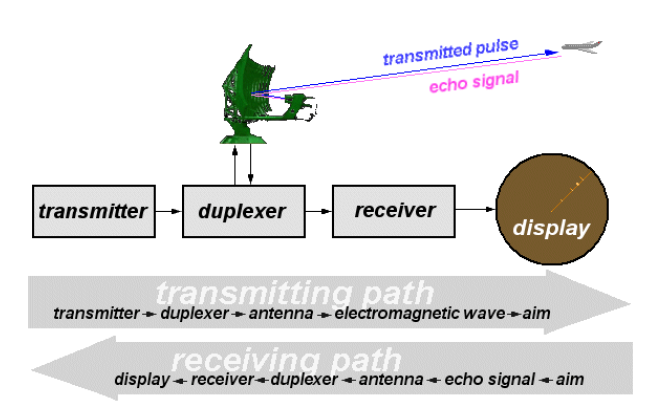
\includegraphics[width=400px, scale=1]{figuras/funcionamento_radar}
  \caption{Esquemático do funcionamento do radar}
\label{fig:funcionamento_radar}
\end{figure}

Os radares funcionam com a emissão de pulsos (transmitted pulses) para posterior detecção dos pulsos refletidos
(echo pulses), isso serve para uma sincronização necessária para a medição de distâncias, já que os pulsos
 são emitidos sequencialmente após um período de tempo (PRT) e os pulsos possuem
  uma largura determinada.

\begin{figure}[h]
  \centering
  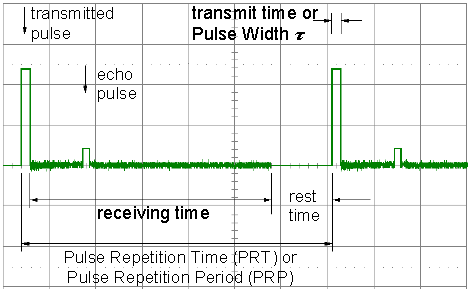
\includegraphics[width=400px, scale=1]{figuras/emissao_pulsos_radar}
  \caption{Gráfico representativo da emissão de pulsos por um radar}
\label{fig:emissao_pulsos_radar}
\end{figure}

A distância entre o radar e o objeto que se quer saber a distância é dada por essa simples equação:

$ R = \displaystyle\frac{Tdelay * C0}{2}$

Onde:

	R: é a distância até o objeto.

	tdelay: é o tempo para o sinal viajar e retornar.

	c0: é a velocidade da luz.

  E as equações para as distâncias máximas e mínimas que um radar pode detectar sem
  causar ambiguidade, sendo trecovery o tempo de recuperação do equipameto
   utilizado, são:


$ Rmax = \frac{(PRT - t) * C0}{2}$

$ Rmin = \frac{(t + Trecovery) * C0}{2}$




Equação teórica do radar:

$p_{r} = \frac{\pi ^{2}p_{t}g^{2}\theta h |K|^{2}l2}{1024ln(2)\lambda ^{2}\gamma ^{2}}$

Onde:

Pt = power transmitted by radar (watts)

Pr = power received back by radar (watts)

g = gain of the antenna (ratio of power on the beam axis to power from an isotropic [i.e.,
radiating equally in all directions] antenna at the same point); it is a measure
of how focused the radar beam is.

$\theta$ = horizontal beamwidth (radians)

$\omega$ = vertical beamwidth (radians)

h = pulselength (m)

|K|2 = dielectric constant for hydrometeors; usually taken as 0.93 for liquid water, 0.197 for
 ice. (Note that for an equivalent mass of frozen precipitation, much less power is returned
 from the ice than from liquid precipitation; thus snow with the same water content is
  less reflective than rain). For this reason, NEXRAD’s clear air mode rather than
  precipitation mode is sometimes used to monitor snow situations because of its greater
  sensitivity).

l = loss factor for attenuation of radar beam, varies between 0 and 1, usually near 1.
 Since the attenuation of the beam is often unknown, it is often ignored.

$\gamma$ = wavelength of radar pulse (m)

r = range or distance to the target (i.e., the distance to an area of precipitation that reflects the originally transmitted pulse back to the radar).

z = radar reflectivity factor (mm6/m3)

\item \textbf{JUSTIFICATIVA DA ESCOLHA}

O radar é um dispositivo amplamente utilizado que possui grande confiabilidade. Várias empresas automotivas utilizam de radares para detecçao de distâncias e velocidades já que se pode ter uma medição precisa e as interferências causadas pelo ambiente ou por condições climáticas poderem, algumas vezes, ser contornados.

\item \textbf{ESPECIFICAÇÕES DO RADAR}
\begin{enumerate}
\item \textbf{Solução fechada}

Radar ARS-30X da Continental.

Performance pode ser vista na Figura \ref{fig:performace_radar}:
\begin{figure}[h]
  \centering
  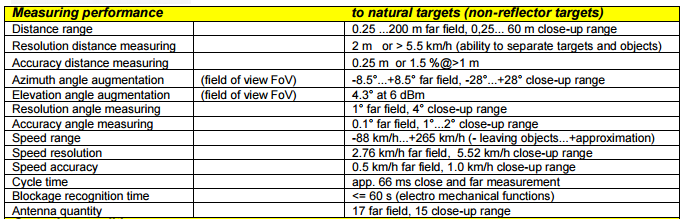
\includegraphics[width=400px, scale=1]{figuras/performace_radar}
  \caption{Performace do Radar ARS}
\label{fig:performace_radar}
\end{figure}

Consumo pode ser vista na Figura \ref{fig:consumo_radar}:
\begin{figure}[h]
  \centering
  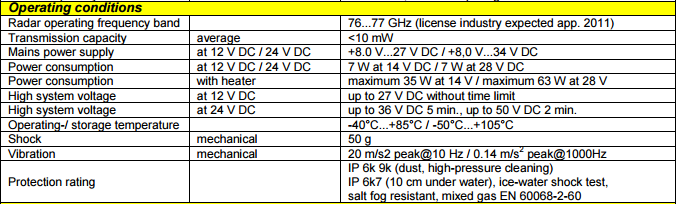
\includegraphics[width=400px, scale=1]{figuras/consumo_radar}
  \caption{Consumo do Radar ARS}
\label{fig:consumo_radar}
\end{figure}

Dimensões pode ser vista na Figura \ref{fig:dimensoes_radar}:
\begin{figure}[h]
  \centering
  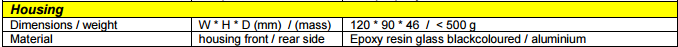
\includegraphics[width=400px, scale=1]{figuras/dimensoes_radar}
  \caption{Dimensões do Radar ARS}
\label{fig:dimensoes_radar}
\end{figure}


\item \textbf{Solução Aberta}
Soluções abertas, a serem definidas pelos equipamentos utilizados em sua produção caso se deseje montar um da
Figura \ref{fig:esquematico_radar}.
\begin{figure}[h]
  \centering
  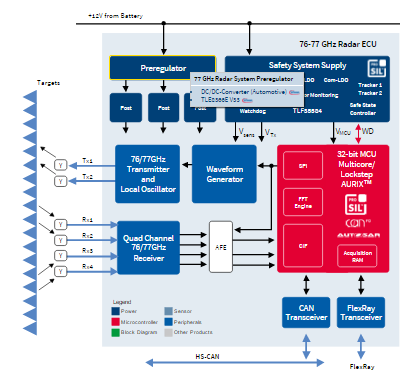
\includegraphics[width=400px, scale=1]{figuras/esquematico_radar}
  \caption{Esquemático dos componentes de um radar}
\label{fig:esquematico_radar}
\end{figure}
\end{enumerate}
\end{enumerate}
